% Figuras del montaje experimental (práctica de muones)
% Requiere en el preámbulo:
%   \usepackage{graphicx}
%   \usepackage{subcaption}
% Ajustar la ruta "figuras/" según dónde estén los PDF.

% ---------------------------------------------------------------- Figura 1
\begin{figure}[htbp]
    \centering
    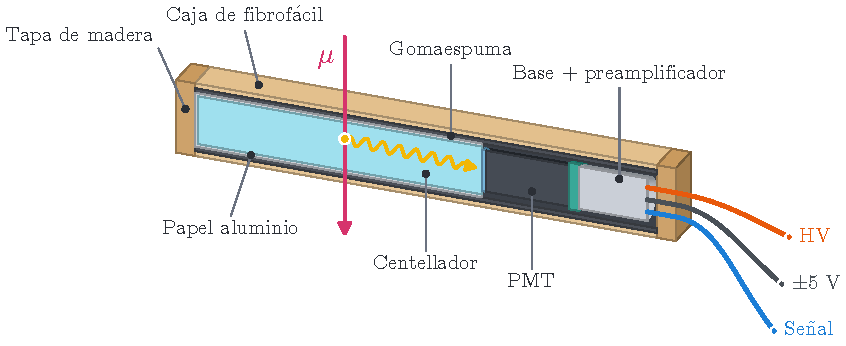
\includegraphics[width=\textwidth]{figuras/fig_modulo.pdf}
    \caption{Corte longitudinal de uno de los módulos detectores. El centellador
    acrílico ($4{,}5 \times 4{,}5 \times 46$~cm) está envuelto en papel aluminio,
    que impide la entrada de luz exterior, y acoplado en uno de sus extremos a un
    fotomultiplicador (PMT). La base del PMT contiene el preamplificador y recibe
    la alta tensión ($-1500$~V) y la alimentación de $\pm 5$~V; por el tercer cable
    sale la señal. El conjunto está protegido con goma espuma negra dentro de una
    caja de fibrofácil cerrada con tapas de madera maciza. Cuando un muón ($\mu$)
    atraviesa el centellador, los fotones de centelleo viajan por el material hasta
    el PMT. La sección transversal está exagerada respecto del largo.}
    \label{fig:modulo}
\end{figure}

% ---------------------------------------------------------------- Figura 2
% Las tres subfiguras van en una fila. Los anchos (0,366 / 0,243 / 0,351)
% son proporcionales al ancho de cada PDF, así las tres quedan a la misma
% escala y con el mismo tamaño de letra (~8 pt con un ancho de texto de 16 cm).
\begin{figure}[htbp]
    \centering
    \begin{subfigure}[b]{0.366\textwidth}
        \centering
        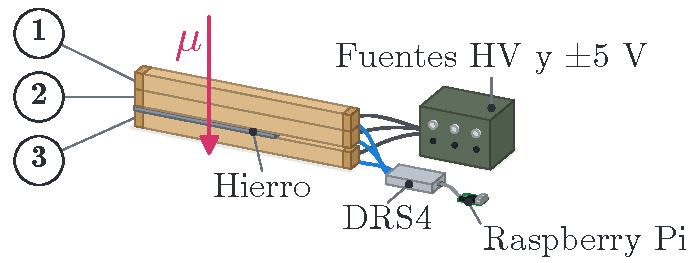
\includegraphics[width=\linewidth]{figuras/disp_apilados.pdf}
        \caption{Apilados con hierro.}
        \label{fig:disp_apilados}
    \end{subfigure}
    \hfill
    \begin{subfigure}[b]{0.243\textwidth}
        \centering
        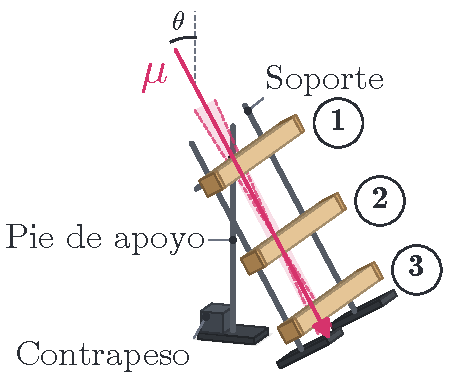
\includegraphics[width=\linewidth]{figuras/disp_inclinados.pdf}
        \caption{Barrido angular.}
        \label{fig:disp_inclinados}
    \end{subfigure}
    \hfill
    \begin{subfigure}[b]{0.351\textwidth}
        \centering
        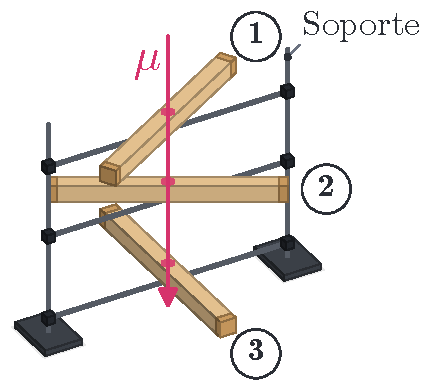
\includegraphics[width=\linewidth]{figuras/disp_velocidades.pdf}
        \caption{Medición de velocidades.}
        \label{fig:disp_velocidades}
    \end{subfigure}

    \caption{Disposiciones experimentales utilizadas. Los números indican cada
    módulo y la flecha, la trayectoria de un muón ($\mu$). Esquemas fuera de escala.
    (a)~Módulos apilados con una placa de hierro entre los módulos 2 y 3, que frena
    a los muones para observar su decaimiento. Las señales de los tres PMT se
    digitalizan con la placa DRS4 (PSI), controlada por una Raspberry Pi.
    (b)~Barrido angular: los módulos se montan en dos soportes (separación entre
    caras superiores de 29,5~cm entre 1 y 2, y de 26,1~cm entre 2 y 3) y la
    estructura se inclina un ángulo $\theta$ respecto de la vertical, apoyada sobre
    un pie con contrapeso. Se midió entre $\theta = -55^\circ$ y $56^\circ$. La
    región sombreada es el cono de trayectorias rectas que atraviesan los tres
    centelladores y determina la incerteza en la dirección de los muones detectados.
    (c)~Medición de velocidades: los módulos se cruzan a $60^\circ$ entre sí sobre
    barras horizontales (separación entre caras superiores de 27,7~cm entre 1 y 2,
    y de 32,5~cm entre 2 y 3), con sus centros sobre una misma vertical. Así solo
    se registran muones prácticamente verticales que atraviesan la zona común a
    los tres centelladores (hexágonos), y el tiempo de propagación de la luz
    dentro de cada centellador es el mismo, por lo que se cancela en las
    diferencias de tiempo.}
    \label{fig:disposiciones}
\end{figure}

% ---------------------------------------------------------------- Figura 3
% Generada con fig_barrido_angular.py (o el notebook analisis/tasa_vs_angulo.ipynb).
\begin{figure}[htbp]
    \centering
    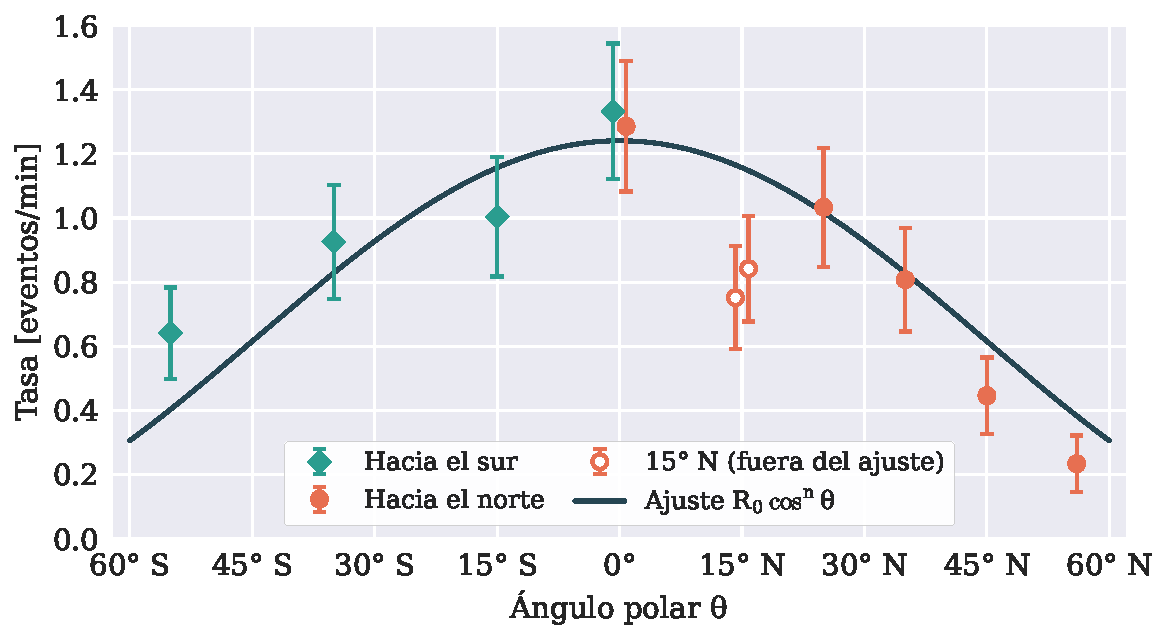
\includegraphics[width=0.85\textwidth]{figuras/barrido_angular.pdf}
    \caption{Tasa de coincidencias triples en función del ángulo polar $\theta$, con
    el telescopio inclinado hacia el sur (rombos) y hacia el norte (círculos). Cada
    punto es una medición de unos 30~min; la tasa es $N/T$, con $N$ el número de
    coincidencias registradas y $T$ el tiempo de medición, y las barras, $\sqrt{N}/T$.
    En $0^\circ$ se midió una vez con cada serie, en días distintos. La curva es el
    ajuste de $R_0\cos^n\theta$ sin las dos mediciones en $15^\circ$~N (símbolos
    huecos): $R_0 = (1{,}24 \pm 0{,}11)$~min$^{-1}$ y $n = 2{,}0 \pm 0{,}4$,
    compatible con el $n \simeq 2$ esperado.}
    \label{fig:barrido_angular}
\end{figure}
